\chapter{CFR-D and Decomposition}
\label{ch:cfr-d}
\note{
  This chapter summarizes the approach, methods and results of~the authors~\cite{BurchJohansonBowling13}.
}

\section{Motivation}
(\cite{BurchJohansonBowling13}) describes a~pioneering technique how to \emph{decompose} subgames of~imperfect-information games and solve them independently, while preserving the optimality of~the full-game solution.
This brings countless benefits:
\begin{itemize}
  \item smarter usage of~run-time information, i.e. endgame actually reached during a~real play
  \item memory and disk limitations
\end{itemize}

\section{Gadget Game}
\epigraphLong{
  Dreams about the future are always filled with gadgets.
}{Neil deGrasse Tyson}
\todo copy-paste

Again, we start by~creating a~fine-grained abstraction for the subgame.
The original strategy for the subgame (from the coarse abstraction) is then translated into the fine-grained abstraction as $\sigma_1^S$.
The translated strategy is now used to compute $CBV_2 ^{\sigma_1^S} (I)$ for every information set~$I$ at~the root of~the subgame.
These values will be useful for the gadget construction to~guarantee the safety of~the resulting strategy.

To construct the gadget, we add one chance node at~the root of~the game, followed by additional nodes for player~$2$:
one for every state at~the root of the subgame.
At~each of~these nodes, $2$ may either accept the corresponding counterfactual best response value calculated earlier, or play the subgame (to get to the corresponding state at~the root of~the subgame).
The chance player distributes the player~$2$ into these states using the (normalized) $\pi^\sigma_{-2}$ (how likely is the state given that $2$ plays to reach it).
Since the game is zero-sum, this forces player~$1$ to play the subgame well enough, so that the opponent's value is no greater than the original CBV.
See Figure~\ref{fig:re-solving-gadget} for a~sketch of~the construction.
For more details see (\cite{BurchJohansonBowling13}).
\begin{figure}[H]
  \centering
  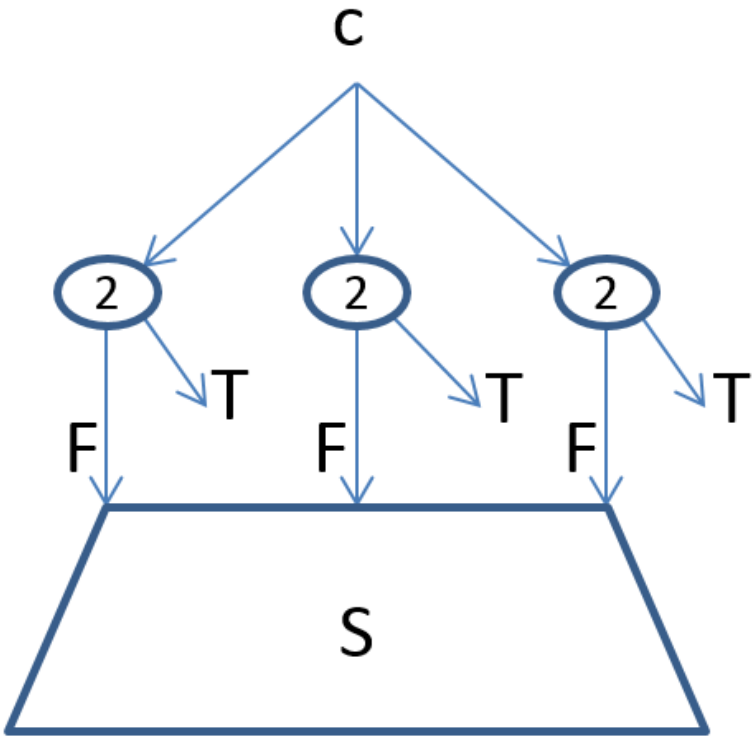
\includegraphics[width=.3\textwidth]{../img/re-solving-game-gadget.png}
  \caption{A~gadget game for re-solving subgames}
  \label{fig:re-solving-gadget}
\end{figure}

\section{Equivalent Linear Program}

\section{Experimental Results}
